% DO NOT COMPILE THIS FILE DIRECTLY!
% This is included by the other .tex files.

\begin{frame}[t,plain]
\titlepage
\end{frame}

\begin{frame}[t]{Computing}
\vskip 1cm
Computing is defined as Counting & Calculating using the devices. The origin of computing started with early man who used fingers, stones, sticks, marks on walls, sand etc. 
\begin{figure}

\includegraphics[height=0.125\paperheight]{tcc}
\end{figure}

\end{frame}

\begin{frame}[t]{Origin of Computing}
Ancient Counting and Calculating devices are :
\begin{itemize}
\item Abacus
\item Napier's Bones
\item Slide Rule
\end{itemize}
\end{frame}

\begin{frame}[t]{Abacus}
\begin{itemize}
\item Developed in 3000 B.C by chinese.
\item Built with wood & beads.
\item Used in schools & shopkeepers.
\end{itemize}
\end{frame}
\begin{frame}[t,fragile]{Napier Bones}
\begin{itemize}
\item In 1617, Napier invented 'Napier's Bones'.
\item Multiplication tables were written on bones, ivory, silver, wood.
\item Simplified multiplication, division, square roots & cube roots.
\end{itemize}
\end{frame}
\begin{frame}[t,fragile]{Python}
\begin{itemize}
\item Dynamic \& powerful programming language.
\item Easy language to work on.
\item High level programming.
\item Platform Independent.
\item OSI-approved open source license.
\item Often used as a scripting language.
\end{itemize}
\end{frame}

\begin{frame}[t,fragile]{Django}
\begin{itemize}
\item Open source web application framework.
\item Written in the Python programming language.
\item Follows the Model View Controller architectural pattern.
\item Ease the creation of complex, database-driven websites.
\item Emphasizes re-usability.
\end{itemize}
\end{frame}

\begin{frame}[t,fragile]{Features of the Software}
\begin{itemize}
\item Open Source
\item User Interactive Software
\item On-line
\item Dynamic
\item Role dependent interface
\item Product/Catalog
\item Distance Calculation through map
\item Search module
\item Universal (Can be changed according to application/work)
\item Report generation
\item Single click installation
\item User and developer documentation

\end{itemize}

\end{frame}
\watermarkoff
{

\begin{frame}[t,fragile]{Work Flow using Software}
\begin{figure}
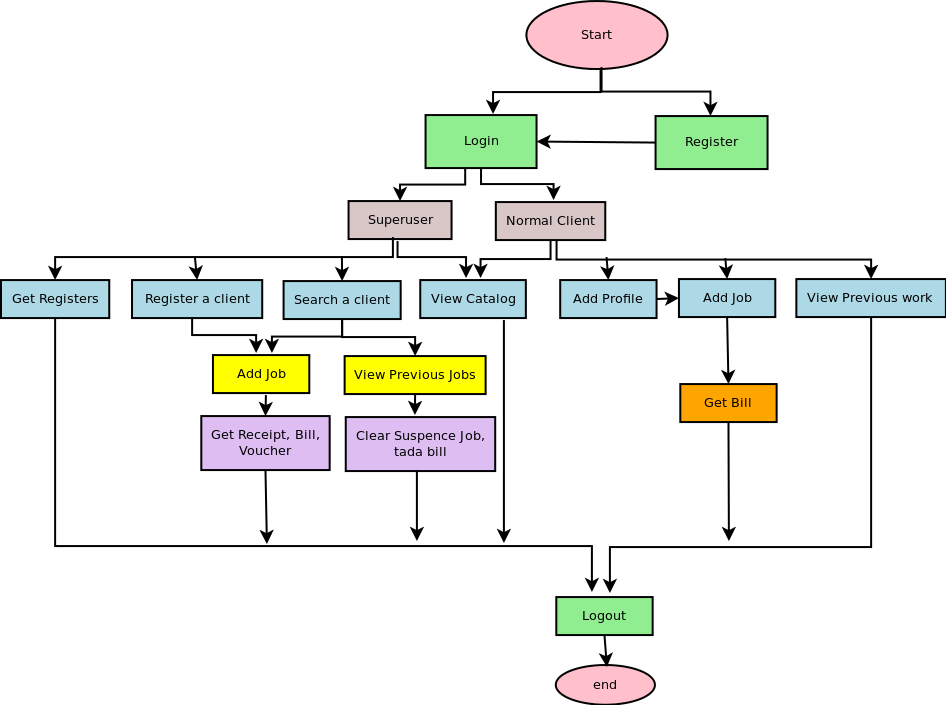
\includegraphics[height=0.6\paperheight]{automation}
\end{figure}
\end{frame}
}

\watermarkon
\begin{frame}[t,fragile]{Future Scope}
Still there are many more things or areas which can
be added to the project to make it more reliable. These remaining areas may be:
\begin{itemize}
\item Receive the payment on-line through e-billing.
\item Managing the labs work through software.
\item SMS Service.
\item Module to fax the documents automatically to the Clients/Employee. 

\end{itemize}
\end{frame}
\watermarkoff
\begin{frame}[t,fragile]{Any Question?}
\begin{figure}

\includegraphics[height=0.7\paperheight]{thank}
\end{figure}
\end{frame}




